\section*{Question 1: Rationality}
\subsection*{(a)}
\uline{Given:} game with pair of dice with 3 possible outcomes
\begin{itemize}
\item throw one six with the pair of dice: +12\euro
\item throw two sixes with the pair of dice: +32\euro
\item throw no six: -8\euro
\end{itemize}
Would you play the game once/twice? Average expected income per round?

There are 36 possible outcomes, how to throw two dices: 
(1,1), (1,2),(1,3),(1,4), (1,5),(1,6),
(2,1), (2,2),(2,3),(2,4), (2,5),(2,6),..., (6,1), (6,2),(6,3),(6,4), (6,5),(2,6).\\
11 of those events contain a six, so there is the opportunity of $\frac{11}{36}$ to throw at least one six.\\
Another approach can be made with a probability tree:\\\\
\begin{minipage}[h]{.45\textwidth}
	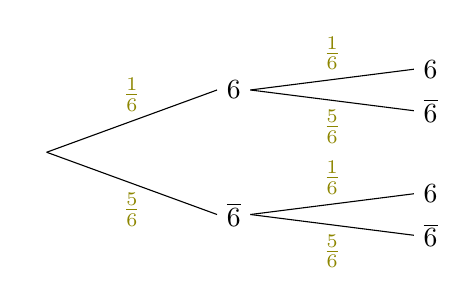
\begin{tikzpicture}[level/.style={level 1/.style={sibling distance=4.5em},
  level 2/.style={sibling distance=1.5em},
  level 3/.style={sibling distance=1em},
  level 4/.style={sibling distance=1em},level distance = 2.5cm}, parent anchor=east,child anchor=west,grow=east]
	\node{}
    child{node{$\overline{6}$}
    	child{node{$\overline{6}$}
        edge from parent node[below,color=olive]{$\frac{5}{6}$}}
    	child{node{6}
        edge from parent node[above,color=olive]{$\frac{1}{6}$}}
        edge from parent node[below,color=olive]{$\frac{5}{6}$}}
	child{node{6}
    	child{node{$\overline{6}$}
        edge from parent node[below,color=olive]{$\frac{5}{6}$}}
    	child{node{6}
        edge from parent node[above,color=olive]{$\frac{1}{6}$}}
        edge from parent node[above,color=olive]{$\frac{1}{6}$}};
	\end{tikzpicture}
\end{minipage}%
\begin{minipage}[h]{.55\textwidth}
The probability to throw exactly one six therefore is $\frac{5}{6}\cdot\frac{1}{6}+\frac{1}{6}\cdot\frac{5}{6} = \frac{5}{36} + \frac{5}{36} = \frac{10}{36}$.\\
The probability to throw two sixes is $\frac{1}{6}\cdot\frac{1}{6}=\frac{1}{36}$. Therefore to probability to win money is $\frac{11}{36}\approx 0.306$, while the probability to lose money is about $\frac{25}{36}\approx 0.694$. As the probability to lose is much higher, it is not in our interest to play the game once. The average expected income per round is $12$\euro$\cdot\frac{10}{36}+32$\euro$\cdot\frac{1}{36}-8$\euro$\cdot\frac{25}{36}=-\frac{4}{3}$\euro, what emphasizes the decision not to play the game. 
\end{minipage}\\\\\\
\begin{minipage}[h]{.8\textwidth}
	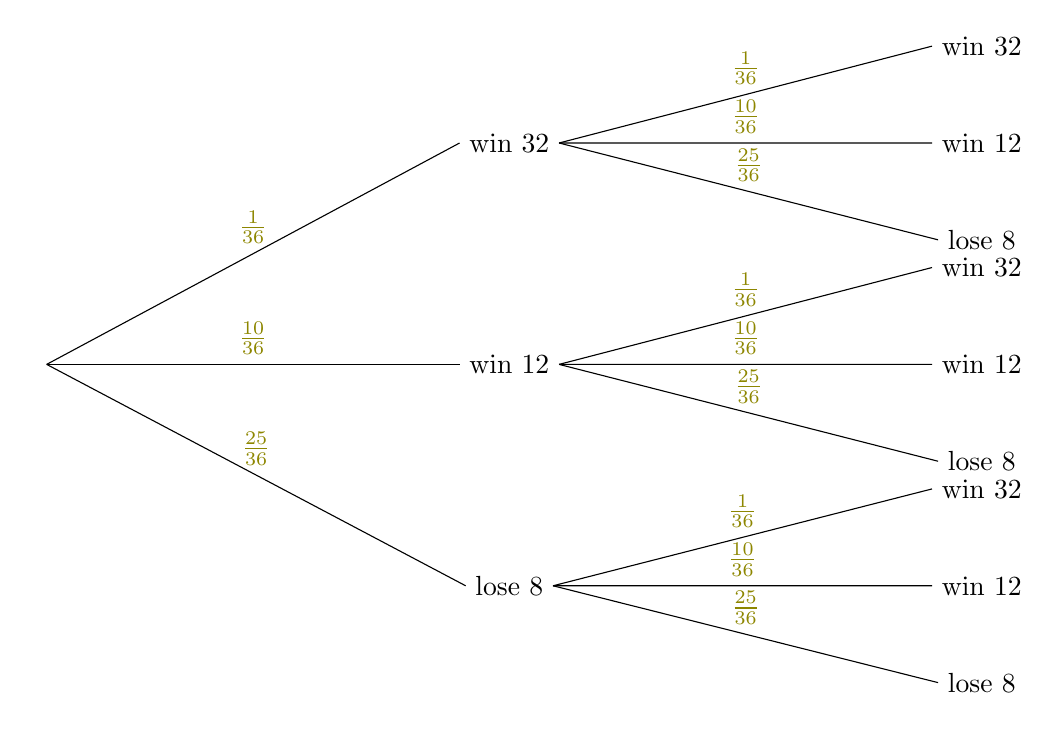
\begin{tikzpicture}[level/.style={level 1/.style={sibling distance=8em},
  level 2/.style={sibling distance=3.5em},
  level 3/.style={sibling distance=2em},level distance = 6cm}, parent anchor=east,child anchor=west,grow=east]
	\node{}
    child{node{lose 8\euro}
    	child{node{lose 8\euro}
        edge from parent node[above,color=olive]{$\frac{25}{36}$}}
        child{node{win 12\euro}
        edge from parent node[above,color=olive]{$\frac{10}{36}$}}
    	child{node{win 32\euro}
        edge from parent node[above,color=olive]{$\frac{1}{36}$}}
        edge from parent node[above,color=olive]{$\frac{25}{36}$}}
    child{node{win 12\euro}
    	child{node{lose 8\euro}
        edge from parent node[above,color=olive]{$\frac{25}{36}$}}
        child{node{win 12\euro}
        edge from parent node[above,color=olive]{$\frac{10}{36}$}}
    	child{node{win 32\euro}
        edge from parent node[above,color=olive]{$\frac{1}{36}$}}
        edge from parent node[above,color=olive]{$\frac{10}{36}$}}
	child{node{win 32\euro}
    	child{node{lose 8\euro}
        edge from parent node[above,color=olive]{$\frac{25}{36}$}}
        child{node{win 12\euro}
        edge from parent node[above,color=olive]{$\frac{10}{36}$}}
    	child{node{win 32\euro}
        edge from parent node[above,color=olive]{$\frac{1}{36}$}}
        edge from parent node[above,color=olive]{$\frac{1}{36}$}};
	\end{tikzpicture}
\end{minipage}\\\\
The probability to win in two rounds can be split up as shown in the probability tree above.
\begin{flalign*}
P(\text{\textit{"win at least once in 2 rounds"}})&=
\underbrace{\frac{1}{36}\cdot\frac{1}{36}}_{\text{win 32\euro  twice}}+
\underbrace{\frac{10}{36}\cdot\frac{10}{36}}_{\text{win 12\euro  twice}}+ \underbrace{2\cdot\frac{1}{36}\cdot\frac{10}{36}}_{\text{win 12+32\euro}}+
\underbrace{2\cdot\frac{1}{36}\cdot\frac{25}{36}}_{\text{win 32-8\euro}}+
\underbrace{2\cdot\frac{10}{36}\cdot\frac{25}{36}}_{\text{win 12-8\euro}}&\\
&=\frac{671}{1296}&\\
&\approx0.5177
\end{flalign*}
The probability to win money after playing the game to rounds is slightly over chance. Therefore it is in our interest to play the game at least two times.
 \newpage
\subsection*{(b)}
Given: 3 exam topics $a$, $b$, $c$ (one easy, two complex)\\
Choose topic, examiner tells you another complex topic\\
Do you want to switch your topic?\\\\
Assuming WLOG he chooses exam $a$ first:\\
Root: Initial Choice ($a$)\\
First level indicates which exam is the actual easy one.\\
Second level indicates which exam the examiner reveals as complex.

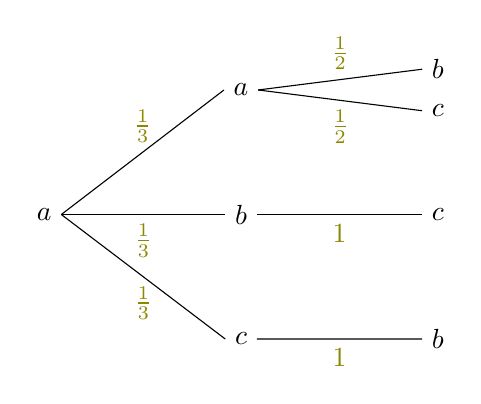
\begin{tikzpicture}[level/.style={level 1/.style={sibling distance=4.5em},
  level 2/.style={sibling distance=1.5em},
  level 3/.style={sibling distance=1em},
  level 4/.style={sibling distance=1em},level distance = 2.5cm}, parent anchor=east,child anchor=west,grow=east]
	\node{$a$}
    child{node{$c$}
   		child{node{$b$}
        edge from parent node[below,color=olive]{$1$}}
        edge from parent node[below,color=olive]{$\frac{1}{3}$}}
    child{node{$b$}
    	child{node{$c$}
        edge from parent node[below,color=olive]{$1$}}
        edge from parent node[below,color=olive]{$\frac{1}{3}$}}
	child{node{$a$}
    	child{node{$c$}
        edge from parent node[below,color=olive]{$\frac{1}{2}$}}
    	child{node{$b$}
        edge from parent node[above,color=olive]{$\frac{1}{2}$}}
        edge from parent node[above,color=olive]{$\frac{1}{3}$}}
    	;
	\end{tikzpicture}
    
\begin{table}[htbp]
\renewcommand{\arraystretch}{1.5}
\begin{tabular}{c | c | c | c | c | c}
Initial Choice & Easy Exam 	& Revealed hard exam	& Probability & Switch & Stay\\ \hline
$a$ & $a$			& $b$						& $\frac{1}{3} \cdot \frac{1}{2} = \frac{1}{6}$ & $c:$ complex & easy\\
~ &~			& $c$						& $\frac{1}{3} \cdot \frac{1}{2} = \frac{1}{6}$ & $b:$ complex & easy  \\ \hline
$a$ & $b$			& $c$						& $\frac{1}{3} \cdot 1 = \frac{1}{3}$ & $b:$ easy & complex\\
\hline
$a$ & $c$			& $b$						& $\frac{1}{3} \cdot 1 = \frac{1}{3}$ & $c:$ easy & complex
\end{tabular}
\end{table}
\begin{enumerate}
\item If you initially pick the exam $a$ and it actually is the easy exam. \\Switching would result in one of the two complex exam.\\
So the probability for switching and getting $a$ hard exam is $\frac{1}{6} + \frac{1}{6} = \frac{1}{3}$
\item If you initially pick the exam $a$ and it actually $a$ complex exam. \\The other complex exam is revealed by the examiner.
\begin{itemize}
	\item So if you switch from the complex exam $a$ to $b$, given the complex exam is $c$, $b$ is the easy exam (Probabilty: $\frac{1}{3} \cdot 1 = \frac{1}{3}$)
    \item So if you switch from the complex exam $a$ to $c$, given the complex exam is $b$, $c$ is the easy exam (Probabilty: $\frac{1}{3} \cdot 1 = \frac{1}{3}$)
\end{itemize}
The whole probability for switching and getting an easy exam is $2 \cdot \frac{1}{3} \cdot 1 = \frac{1}{3} = \frac{2}{3}$	\\
\end{enumerate}
$\Rightarrow$  Yes, it is in my advantage, to switch because the probability for switching and getting an easy exam equals $\frac{2}{3}$, while the probability for staying and getting an easy exam equals $\frac{1}{3}$.


\section*{Question 2: Search strategies}
\subsection*{(a) Breadth-first search}
\begin{minipage}[t]{.8\textwidth}
	\centering
	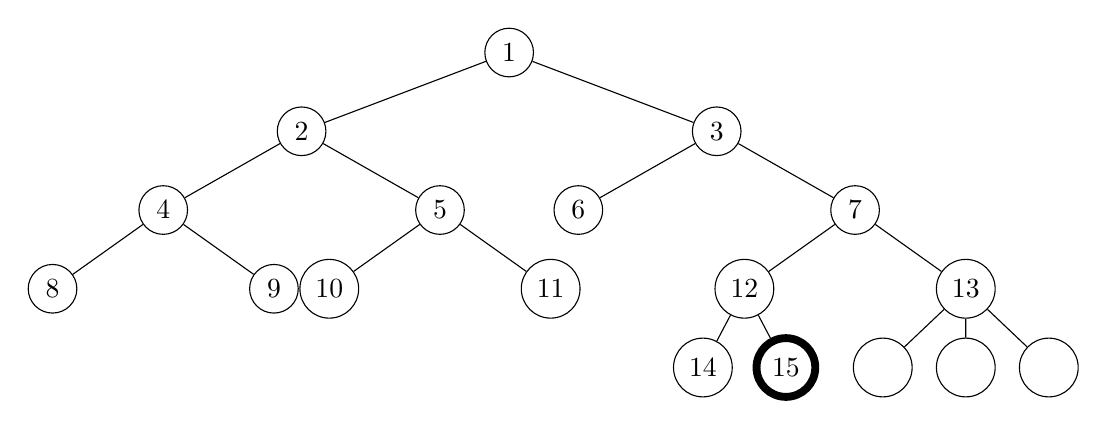
\begin{tikzpicture}[level/.style={level 1/.style={sibling distance=15em},
  level 2/.style={sibling distance=10em},
  level 3/.style={sibling distance=8em},
  level 4/.style={sibling distance=3em},level distance = 1cm}]
	\node[circle,draw]{1}
	child{node[circle,draw]{2}
    	child{node[circle,draw]{4}
        	child{node[circle,draw]{8}}
            child{node[circle,draw]{9}}}
        child{node[circle,draw]{5}
        	child{node[circle,draw]{10}}
            child{node[circle,draw]{11}}}}
	child{node[circle,draw]{3}
    	child{node[circle,draw]{6}}
        child{node[circle,draw]{7}
        	child{node[circle,draw]{12}
            	child{node[circle,draw]{14}}
            	child{node[circle,line width=1mm, draw]{15}}}
            child{node[circle,draw]{13}
            	child{node[circle,draw]{\textcolor{white}{10}}}
            	child{node[circle,draw]{\textcolor{white}{10}}}
                child{node[circle,draw]{\textcolor{white}{10}}}}}};
	\end{tikzpicture}
\end{minipage}
\subsection*{(b) Depth-first search}
\begin{minipage}[t]{.8\textwidth}
	\centering
	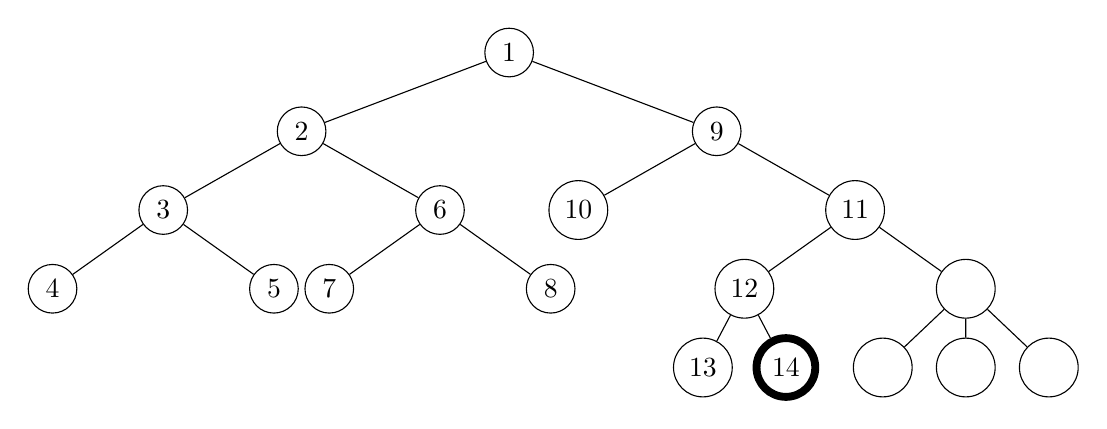
\begin{tikzpicture}[level/.style={level 1/.style={sibling distance=15em},
  level 2/.style={sibling distance=10em},
  level 3/.style={sibling distance=8em},
  level 4/.style={sibling distance=3em},level distance = 1cm}]
	\node[circle,draw]{1}
	child{node[circle,draw]{2}
    	child{node[circle,draw]{3}
        	child{node[circle,draw]{4}}
            child{node[circle,draw]{5}}}
        child{node[circle,draw]{6}
        	child{node[circle,draw]{7}}
            child{node[circle,draw]{8}}}}
	child{node[circle,draw]{9}
    	child{node[circle,draw]{10}}
        child{node[circle,draw]{11}
        	child{node[circle,draw]{12}
            	child{node[circle,draw]{13}}
            	child{node[circle,line width=1mm, draw]{14}}}
            child{node[circle,draw]{\textcolor{white}{10}}
            	child{node[circle,draw]{\textcolor{white}{10}}}
            	child{node[circle,draw]{\textcolor{white}{10}}}
                child{node[circle,draw]{\textcolor{white}{10}}}}}};
	\end{tikzpicture}
\end{minipage}
\subsection*{(c) Iterative deepening depth-first search}
\begin{minipage}[t]{.5\textwidth}
\flushleft{\uline{Depth limit = 1}}\\
	\centering
    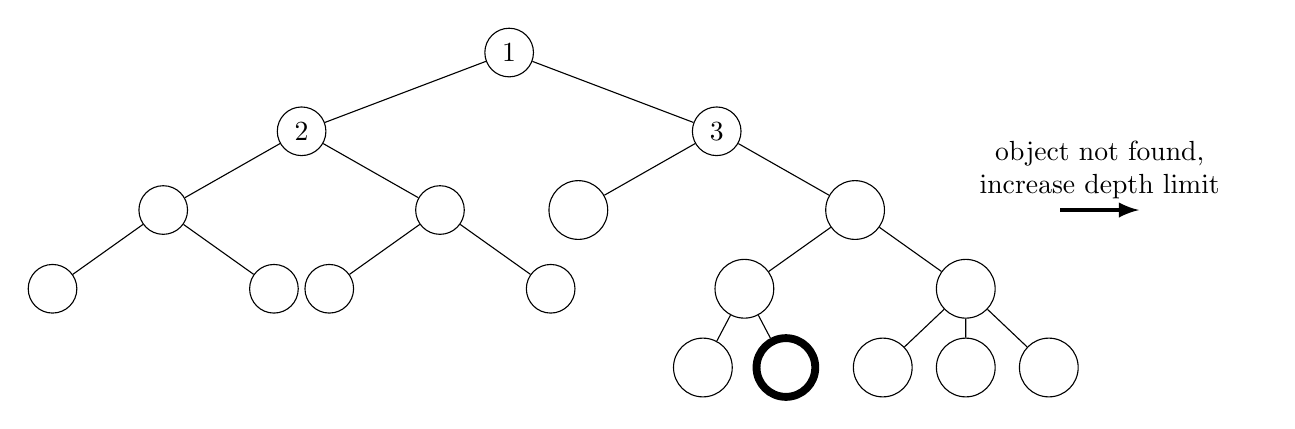
\begin{tikzpicture}[level/.style={level 1/.style={sibling distance=15em},
  level 2/.style={sibling distance=10em},
  level 3/.style={sibling distance=8em},
  level 4/.style={sibling distance=3em},level distance = 1cm}]
	\node[circle,draw]{1}
	child{node[circle,draw]{2}
    	child{node[circle,draw]{\textcolor{white}{1}}
        	child{node[circle,draw]{\textcolor{white}{1}}}
            child{node[circle,draw]{\textcolor{white}{1}}}}
        child{node[circle,draw]{\textcolor{white}{1}}
        	child{node[circle,draw]{\textcolor{white}{1}}}
            child{node[circle,draw]{\textcolor{white}{1}}}}}
	child{node[circle,draw]{3}
    	child{node[circle,draw]{\textcolor{white}{10}}}
        child{node[circle,draw]{\textcolor{white}{10}}
        	child{node[circle,draw]{\textcolor{white}{10}}
            	child{node[circle,draw]{\textcolor{white}{10}}}
            	child{node[circle,line width=1mm, draw]{\textcolor{white}{10}}}}
            child{node[circle,draw]{\textcolor{white}{10}}
            	child{node[circle,draw]{\textcolor{white}{10}}}
            	child{node[circle,draw]{\textcolor{white}{10}}}
                child{node[circle,draw]{\textcolor{white}{10}}}}}};
\draw[line width=1.5pt, ->, >=latex]
	(7, -2) -- (8, -2) node [midway, above, text width = 4cm, align = center]  {object not found, increase depth limit};
	\end{tikzpicture}
\end{minipage}\\
\begin{minipage}[t]{.5\textwidth}
\flushleft{\uline{Depth limit = 2}}\\
	\centering
	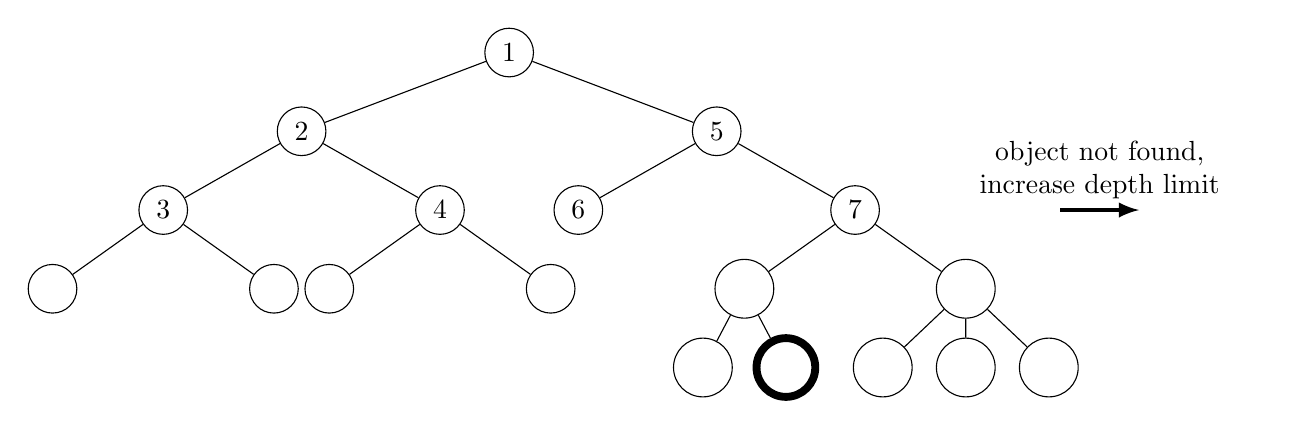
\begin{tikzpicture}[level/.style={level 1/.style={sibling distance=15em},
  level 2/.style={sibling distance=10em},
  level 3/.style={sibling distance=8em},
  level 4/.style={sibling distance=3em},level distance = 1cm}]
	\node[circle,draw]{1}
	child{node[circle,draw]{2}
    	child{node[circle,draw]{3}
        	child{node[circle,draw]{\textcolor{white}{1}}}
            child{node[circle,draw]{\textcolor{white}{1}}}}
        child{node[circle,draw]{4}
        	child{node[circle,draw]{\textcolor{white}{1}}}
            child{node[circle,draw]{\textcolor{white}{1}}}}}
	child{node[circle,draw]{5}
    	child{node[circle,draw]{6}}
        child{node[circle,draw]{7}
        	child{node[circle,draw]{\textcolor{white}{10}}
            	child{node[circle,draw]{\textcolor{white}{10}}}
            	child{node[circle,line width=1mm, draw]{\textcolor{white}{10}}}}
            child{node[circle,draw]{\textcolor{white}{10}}
            	child{node[circle,draw]{\textcolor{white}{10}}}
            	child{node[circle,draw]{\textcolor{white}{10}}}
                child{node[circle,draw]{\textcolor{white}{10}}}}}};
\draw[line width=1.5pt, ->, >=latex]
	(7, -2) -- (8, -2) node [midway, above, text width = 4cm, align = center]  {object not found, increase depth limit};
	\end{tikzpicture}
\end{minipage}\\
\begin{minipage}[t]{.5\textwidth}
\flushleft{\uline{Depth limit = 3}}\\
	\centering
	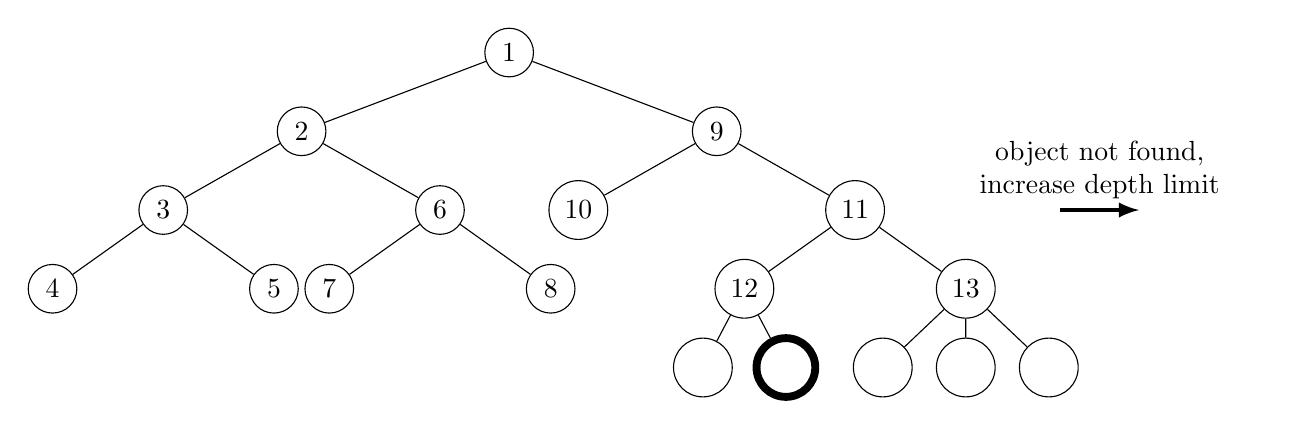
\begin{tikzpicture}[level/.style={level 1/.style={sibling distance=15em},
  level 2/.style={sibling distance=10em},
  level 3/.style={sibling distance=8em},
  level 4/.style={sibling distance=3em},level distance = 1cm}]
	\node[circle,draw]{1}
	child{node[circle,draw]{2}
    	child{node[circle,draw]{3}
        	child{node[circle,draw]{4}}
            child{node[circle,draw]{5}}}
        child{node[circle,draw]{6}
        	child{node[circle,draw]{7}}
            child{node[circle,draw]{8}}}}
	child{node[circle,draw]{9}
    	child{node[circle,draw]{10}}
        child{node[circle,draw]{11}
        	child{node[circle,draw]{12}
            	child{node[circle,draw]{\textcolor{white}{10}}}
            	child{node[circle,line width=1mm, draw]{\textcolor{white}{10}}}}
            child{node[circle,draw]{13}
            	child{node[circle,draw]{\textcolor{white}{10}}}
            	child{node[circle,draw]{\textcolor{white}{10}}}
                child{node[circle,draw]{\textcolor{white}{10}}}}}};
\draw[line width=1.5pt, ->, >=latex]
	(7, -2) -- (8, -2) node [midway, above, text width = 4cm, align = center]  {object not found, increase depth limit};
	\end{tikzpicture}
\end{minipage}\\
\begin{minipage}[t]{.5\textwidth}
\flushleft{\uline{Depth limit = 4}}\\
	\centering
	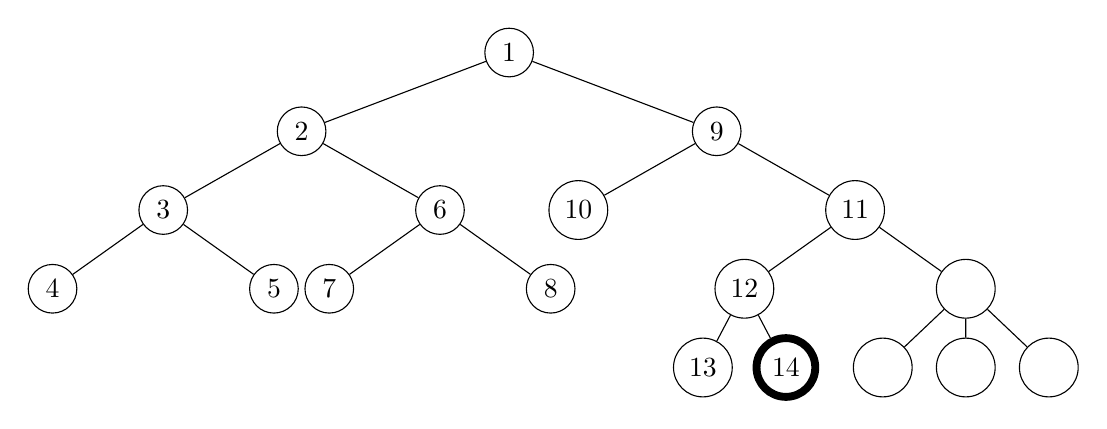
\begin{tikzpicture}[level/.style={level 1/.style={sibling distance=15em},
  level 2/.style={sibling distance=10em},
  level 3/.style={sibling distance=8em},
  level 4/.style={sibling distance=3em},level distance = 1cm}]
	\node[circle,draw]{1}
	child{node[circle,draw]{2}
    	child{node[circle,draw]{3}
        	child{node[circle,draw]{4}}
            child{node[circle,draw]{5}}}
        child{node[circle,draw]{6}
        	child{node[circle,draw]{7}}
            child{node[circle,draw]{8}}}}
	child{node[circle,draw]{9}
    	child{node[circle,draw]{10}}
        child{node[circle,draw]{11}
        	child{node[circle,draw]{12}
            	child{node[circle,draw]{13}}
            	child{node[circle,line width=1mm, draw]{14}}}
            child{node[circle,draw]{\textcolor{white}{10}}
            	child{node[circle,draw]{\textcolor{white}{10}}}
            	child{node[circle,draw]{\textcolor{white}{10}}}
                child{node[circle,draw]{\textcolor{white}{10}}}}}};
	\end{tikzpicture}
\end{minipage}
\section*{Question 3: Programming in LISP}
(see LISP-Code in Bott\_Gorecki\_Assignment02Q3.txt)